% Performance of the wsq-viewer WSQ codec: optimizations, exactness, backends and a GPU test.
% Build: latexmk (see latexmkrc; LuaLaTeX).
\documentclass[11pt,a4paper]{article}

\usepackage[a4paper,textwidth=15cm,top=2.8cm,bottom=3cm]{geometry}
\usepackage{amsmath}
\usepackage{fontspec}
\usepackage{unicode-math}
\setmainfont{EB Garamond}[Numbers={Lining,Proportional}]
\setmathfont{Garamond-Math.otf}
\setmonofont{Inconsolatazi4}[Scale=MatchLowercase,
  UprightFont=*-Regular, BoldFont=*-Bold, Extension=.otf]
\usepackage{microtype}

\usepackage{graphicx}
\usepackage{booktabs}
\usepackage{array}
\usepackage{enumitem}
\setlist{nosep,leftmargin=*,labelindent=\parindent}
\usepackage[font=small,labelfont=sc,labelsep=period]{caption}

\usepackage{tikz}
\usetikzlibrary{arrows.meta,positioning,calc,fit,decorations.pathreplacing,patterns}
\tikzset{
  >={Stealth[length=2.2mm]},
  every picture/.style={line width=0.5pt},
  box/.style={draw,minimum height=7mm,minimum width=14mm,inner sep=2pt},
}
\usepackage{pgfplots}
\pgfplotsset{compat=1.18}

\usepackage{algorithm}
\usepackage[noend]{algpseudocode}
\algrenewcommand\algorithmicrequire{\textit{Input:}}
\algrenewcommand\algorithmicensure{\textit{Output:}}
\algrenewcommand\alglinenumber[1]{\footnotesize #1}
\algrenewcommand{\algorithmiccomment}[1]{\hfill\textit{#1}}

\usepackage[hidelinks]{hyperref}

\newcommand{\marker}[1]{\texttt{#1}}
\newcommand{\code}[1]{\texttt{#1}}
\newcommand{\floor}[1]{\lfloor #1 \rfloor}

% this report is mostly tables: let a page hold more of them
\renewcommand{\topfraction}{0.85}
\renewcommand{\textfraction}{0.1}
\setcounter{topnumber}{3}
\setcounter{totalnumber}{4}

\title{Making WSQ Fast\\[0.4em]
  \large Optimizations, exactness and backends of the \texttt{wsq-viewer} codec,\\
  measured against NBIS 5.0.0}
\author{João Felipe Contreras\\\small\texttt{github.com/JF235/wsq-viewer}}
\date{November 2026}

\begin{document}
\maketitle

\begin{abstract}
\noindent
This report describes how the WSQ codec of the \texttt{wsq-viewer} project was made fast
without giving up exactness, and measures it. The codec is written in Rust and runs natively
and in WebAssembly. In its exact mode it reproduces the NIST reference implementation (NBIS)
bit for bit: the decoder outputs the same pixels and the encoder writes the same bytes on all
86 decoder files and all 80 encoder cases of the NIST compliance set, on every instruction set
and with any number of threads. The algorithms are written once, generically, over a small
vector interface; backends implement that interface for scalar code, SSE2, AVX2 with FMA,
AVX-512 and WebAssembly SIMD. We report the gain of each optimization, compare against NBIS,
check whether relaxing bit exactness buys more speed, and test a GPU for batch decoding.
\end{abstract}

\setcounter{tocdepth}{1}
\tableofcontents

\section{Introduction}
\label{sec:introduction}

The \texttt{wsq-viewer} project needs a WSQ codec that runs inside Visual Studio Code, without
Python or native dependencies, fast enough that opening a fingerprint feels instantaneous, and
correct enough to be trusted for forensic images. The companion document \emph{The WSQ
Fingerprint Image Compression Algorithm} describes the algorithm; this one describes how its
implementation was made fast and how fast it is.

The codec is a Rust library (\code{crates/wsq}) with a command-line tool and a WebAssembly
build for the extension. It has two arithmetic contracts:
\begin{description}[leftmargin=0pt]
  \item[Exact mode] reproduces NBIS 5.0.0, the NIST reference implementation, bit for bit: the
    decoder returns exactly the pixels of \code{dwsq}, and the encoder writes exactly the bytes of
    \code{cwsq}, comment included.
  \item[Fast mode] lets the arithmetic run in any order, with fused multiply-add and double
    precision where cheaper, and stays within the compliance tolerances of the specification.
\end{description}
Both modes run on any of five instruction sets, selected at run time.

Table~\ref{tab:summary} summarizes the outcome on a 1452$\times$1006 four-finger slap
compressed at 0.75 bits per pixel, on one performance core of a 2022 laptop processor. The rest
of the report explains how these numbers were obtained (Sections~\ref{sec:method}
to~\ref{sec:optimizations}), presents the measurements on the whole NIST data set
(Section~\ref{sec:results}), answers whether giving up exactness would buy more speed
(Section~\ref{sec:relaxation}), and reports a test of batch decoding on a GPU
(Section~\ref{sec:gpu}).

% Generated by tools/gen_tables.py; do not edit by hand.
\begin{table}[ht]
  \centering\small
  \begin{tabular}{@{}lrrrr@{}}
    \toprule
    & \multicolumn{2}{c}{decode} & \multicolumn{2}{c}{encode}\\
    \cmidrule(lr){2-3}\cmidrule(l){4-5}
    implementation & ms & vs NBIS & ms & vs NBIS\\
    \midrule
    NBIS 5.0.0 (C), one core & 52.38 & 1.0$\times$ & 36.74 & 1.0$\times$\\
    scalar, exact & 9.77 & 5.4$\times$ & -- & --\\
    SSE2, exact & 7.15 & 7.3$\times$ & -- & --\\
    AVX2, exact & 4.80 & 10.9$\times$ & 6.94 & 5.3$\times$\\
    AVX2, fast & 4.49 & 11.7$\times$ & 7.09 & 5.2$\times$\\
    AVX2, exact, 4 threads & 2.66 & 19.7$\times$ & -- & --\\
    WebAssembly in Node.js, scalar, exact & 18.67 & 2.8$\times$ & -- & --\\
    WebAssembly in Node.js, SIMD, exact & 6.50 & 8.1$\times$ & -- & --\\
    \bottomrule
  \end{tabular}
  \caption{Image \texttt{a002} of the NIST set (1452$\times$1006, a four-finger slap) at 0.75 bits per pixel: median times. Exact means the same pixels and bytes as NBIS.}
  \label{tab:summary}
\end{table}


\section{How the measurements were made}
\label{sec:method}

\paragraph*{Machine.} % Generated by tools/gen_tables.py; do not edit by hand.
An 12th Gen Intel Core i5-12450H laptop processor; Rust 1.92.0, Node.js 24.10.0, gcc 13.3.0 for NBIS.
 The processor has four performance cores
(two threads each) and four efficiency cores; it has AVX2 and FMA but not AVX-512;
Section~\ref{sec:server} repeats the single-core measurements on a server processor that has it.
Single-thread measurements run pinned to one performance core (\code{taskset -c 2}); the
multi-threaded ones use the performance cores, and the batch measurements all twelve hardware
threads. The GPU is the laptop's NVIDIA GeForce RTX 3050 (6 GB).

\paragraph*{Data.} The 40 images of the NIST WSQ reference data set version 2.0 (rolled prints,
plain impressions and four-finger slaps, from 375$\times$526 to 1600$\times$1500 pixels). For
decoding, the inputs are the streams NBIS writes for those images at 0.75 and at 2.25 bits per
pixel, 80 files in all; the 86 files NIST distributes for decoder testing were used for the
correctness checks but not for timing, because their Huffman tables make NBIS print a warning
per table, which would add console output to its times.

\paragraph*{Reference.} NBIS 5.0.0, compiled with its own build system (\code{gcc -O2}), timed
in memory through \code{wsq\_decode\_mem} and \code{wsq\_encode\_mem} by a small C harness
(\code{bench/nbis}). Our codec is timed in memory as well (\code{wsq bench}); file reading and
writing are excluded on both sides.

\paragraph*{Statistic.} Every time is the median of 9 runs (5 for encoding) after one warm-up
run; the decoder and encoder reuse their buffers across runs, as a program decoding many images
would. Per-stage times come from timestamps inside the codec.

\paragraph*{What \emph{faster} means here.} The rows of Tables~\ref{tab:decode}
and~\ref{tab:encode} add up the per-image medians over the 40 images of a set; speedups are
ratios of those sums, so large images weigh more than small ones, as they do in practice.

\section{Algorithms and backends}
\label{sec:architecture}

The codec separates \emph{what} is computed from \emph{how} it is executed
(Figure~\ref{fig:architecture}). Every numerically heavy step is a kernel written once, in
generic Rust, over a vector type \code{V}. The kernels know the algorithm (the operation order
of a transform schedule, the dequantization formula, the run-length scan of the tokenizer) but
nothing about instruction sets. A \emph{backend} is an implementation of the trait \code{Vf32}:
about twenty primitive operations on a vector of float32 lanes (Table~\ref{tab:primitives}).
Adding an instruction set means implementing those primitives, not rewriting the codec.

\begin{figure}[ht]
  \centering
  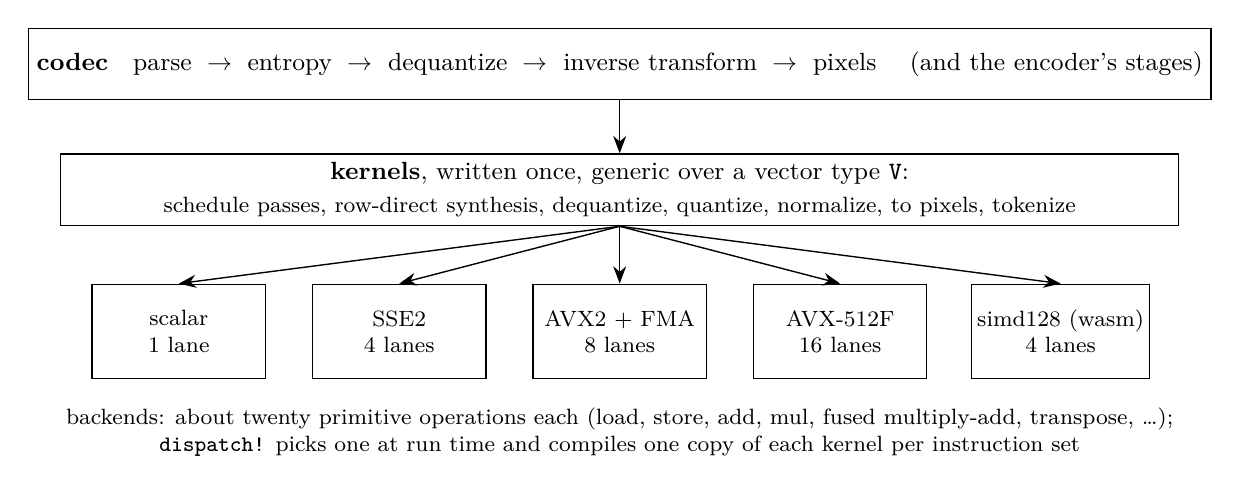
\begin{tikzpicture}[font=\small,
    layer/.style={draw,minimum height=9mm,align=center,inner sep=3pt},
    be/.style={draw,minimum height=12mm,minimum width=22mm,align=center,inner sep=2pt,font=\footnotesize}]
  % codec stages
  \node[layer,minimum width=14.2cm] (codec) at (0,3.2)
    {\textbf{codec}\quad parse \;$\to$\; entropy \;$\to$\; dequantize \;$\to$\; inverse transform \;$\to$\; pixels
     \quad(and the encoder's stages)};
  % kernels
  \node[layer,minimum width=14.2cm] (kern) at (0,1.6)
    {\textbf{kernels}, written once, generic over a vector type \code{V}:\\[1pt]
     \footnotesize schedule passes, row-direct synthesis, dequantize, quantize, normalize, to pixels, tokenize};
  % backends
  \node[be] (s) at (-5.6,-0.2) {scalar\\1 lane};
  \node[be] (sse) at (-2.8,-0.2) {SSE2\\4 lanes};
  \node[be] (avx) at (0,-0.2) {AVX2 + FMA\\8 lanes};
  \node[be] (avx5) at (2.8,-0.2) {AVX-512F\\16 lanes};
  \node[be] (w) at (5.6,-0.2) {simd128 (wasm)\\4 lanes};
  \node[font=\footnotesize,align=center,anchor=north] at (0,-1.05)
    {backends: about twenty primitive operations each (load, store, add, mul, fused multiply-add, transpose, \dots);\\
     \code{dispatch!} picks one at run time and compiles one copy of each kernel per instruction set};
  \draw[->] (codec) -- (kern);
  \foreach \b in {s,sse,avx,avx5,w} \draw[->] (kern.south) -- (\b.north);
\end{tikzpicture}

  \caption{Algorithms and backends. The codec calls kernels; the kernels are generic over the
  vector type; one implementation of the vector type exists per instruction set.}
  \label{fig:architecture}
\end{figure}

\begin{table}[ht]
  \centering\small
  \begin{tabular}{@{}lp{10.3cm}@{}}
    \toprule
    primitive & use \\
    \midrule
    \code{load}, \code{store}, \code{splat} & moving data; broadcasting a coefficient \\
    \code{add}, \code{sub}, \code{mul}, \code{div} & IEEE float32 arithmetic, identical on every backend \\
    \code{fmadd} & $a b + c$, fused where the hardware has FMA (fast mode only) \\
    \code{transpose} & a LANES$\times$LANES block (row passes of the analysis) \\
    \code{interleave} & merges even and odd outputs (row-direct synthesis) \\
    \code{min}, \code{max}, \code{trunc}, \code{select\_gt} & clamping, quantization \\
    \code{copysign}, \code{where\_nonzero} & dequantization without branches \\
    \code{from\_u8}, \code{store\_u8} & pixel conversion in and out \\
    \code{nonzero\_bits} & skipping zeros eight or sixteen at a time in the tokenizer \\
    \bottomrule
  \end{tabular}
  \caption{The vector interface. Each backend implements these operations with its intrinsics:
  \code{\_mm\_*} (SSE2), \code{\_mm256\_*} (AVX2 and FMA), \code{\_mm512\_*} (AVX-512F) or
  \code{f32x4\_*} (WebAssembly SIMD); the scalar backend uses plain Rust.}
  \label{tab:primitives}
\end{table}

\subsection{Dispatch}

Only inside a function that carries the attribute \code{\#[target\_feature]} does Rust
compile code for a given instruction set. A macro, \code{dispatch!}, turns each generic entry point into one
such wrapper per backend and selects one at run time from the CPU's features
(Algorithm~\ref{alg:dispatch}). The generic code is inlined into each wrapper, so the
intrinsics of the backend are inlined too, with no call per operation. One subtlety cost a
factor of ten during development: closures do not inherit target features, so a kernel called
from inside a thread's closure ran with every vector operation as a function call. Each thread
now dispatches on its own.

\begin{algorithm}[ht]
  \caption{Dispatch of a generic kernel (simplified from \code{simd.rs}).}
  \label{alg:dispatch}
  \begin{algorithmic}[1]
    \Function{Run}{backend, args}
      \If{backend $=$ AVX2}
        \State \code{\#[target\_feature(enable = "avx2,fma")]}
        \State \textbf{define} \Call{Wrapper}{args}: \Return \Call{Kernel}{$\langle$Avx2$\rangle$, args}
        \State \Return \Call{Wrapper}{args}
      \ElsIf{backend $=$ AVX-512} \Comment{likewise with \code{avx512f}}
      \ElsIf{backend $=$ SSE2} \Comment{likewise with \code{sse2}}
      \Else\ \Return \Call{Kernel}{$\langle$Scalar$\rangle$, args}
      \EndIf
    \EndFunction
  \end{algorithmic}
\end{algorithm}

The library picks the widest available backend unless told otherwise; the command-line tool
and the tests can force one. WebAssembly has no run-time detection: the extension ships the
module compiled with \code{simd128}, which every current browser engine and Node.js support.

\section{Exactness}
\label{sec:exactness}

Floating-point addition is not associative, so two correct implementations of the same
formula usually differ in the last bits, and after rounding to 8 bits a few pixels differ by
one grey level. The WSQ specification tolerates that (at least 99.9\% of the pixels equal and
none off by more than one), but a viewer that shows exactly what the reference decoder shows
removes any doubt, and an encoder that writes the reference's bytes can be checked with a
hash. Exactness had to coexist with vectorization; this section shows how.

\subsection{Recording the operation order}

The inverse transform of NBIS walks a pointer back and forth over each line, reflecting at the
ends, and accumulates products in a particular order. Rather than re-deriving that order, the
codec contains a literal port of the two NBIS routines (\code{get\_lets} and \code{join\_lets})
that, instead of computing, \emph{records} for every output sample the list of
(input index, coefficient) pairs in the order NBIS adds them, including the cases where NBIS
overwrites a partial sum. The result is a \emph{schedule} per line length and parity. Evaluating
a schedule in float32, multiply then add, never fused, reproduces NBIS bit for bit; the schedules
are computed once per image size and cached.

Exactness then constrains the order of operations \emph{within} one output, not across outputs.
A vector can therefore hold several lines at once: in the column pass, eight adjacent columns
for AVX2 (Figure~\ref{fig:lanes}); every lane performs exactly the scalar sequence of its line.
For the row pass, the codec detects, from the schedule itself, the long interior run in which
consecutive even outputs (and consecutive odd ones) use the same terms shifted by one sample.
There a vector holds consecutive outputs of the same row, and an interleave merges even and odd
results (Figure~\ref{fig:rowdirect}). The few outputs near the ends of a row, whose terms differ,
are evaluated one at a time from the schedule.

\begin{figure}[ht]
  \centering
  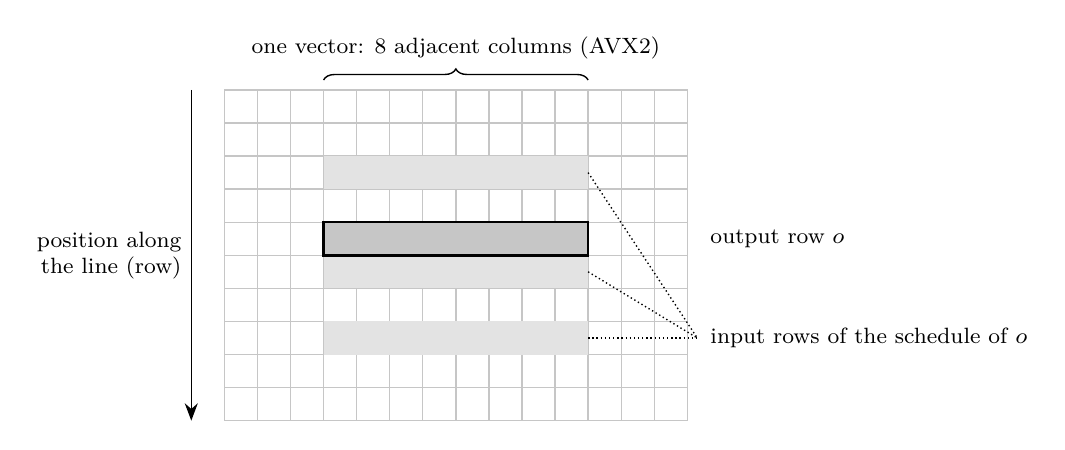
\begin{tikzpicture}[x=0.42cm,y=-0.42cm,font=\footnotesize]
  % a region: columns are lines of the column pass
  \foreach \c in {0,...,13} \foreach \r in {0,...,9} \draw[gray!45] (\c,\r) rectangle (\c+1,\r+1);
  \fill[gray!22] (3,2) rectangle (11,3);
  \fill[gray!22] (3,5) rectangle (11,6);
  \fill[gray!22] (3,7) rectangle (11,8);
  \fill[gray!45] (3,4) rectangle (11,5);
  \draw[line width=0.9pt] (3,4) rectangle (11,5);
  \draw[decorate,decoration={brace,amplitude=4pt}] (3,-0.3) -- (11,-0.3) node[midway,above=4pt] {one vector: 8 adjacent columns (AVX2)};
  \draw[->] (-1,0) -- (-1,10) node[midway,left,align=right] {position along\\the line (row)};
  \node[anchor=west] at (14.4,4.5) {output row $o$};
  \node[anchor=west] at (14.4,7.5) {input rows of the schedule of $o$};
  \draw[densely dotted] (11,2.5) -- (14.3,7.5);
  \draw[densely dotted] (11,5.5) -- (14.3,7.5);
  \draw[densely dotted] (11,7.5) -- (14.3,7.5);
\end{tikzpicture}

  \caption{Column pass: one vector covers adjacent columns, each lane runs the schedule of its
  column, so the operation order of every output is the scalar one.}
  \label{fig:lanes}
\end{figure}

\begin{figure}[ht]
  \centering
  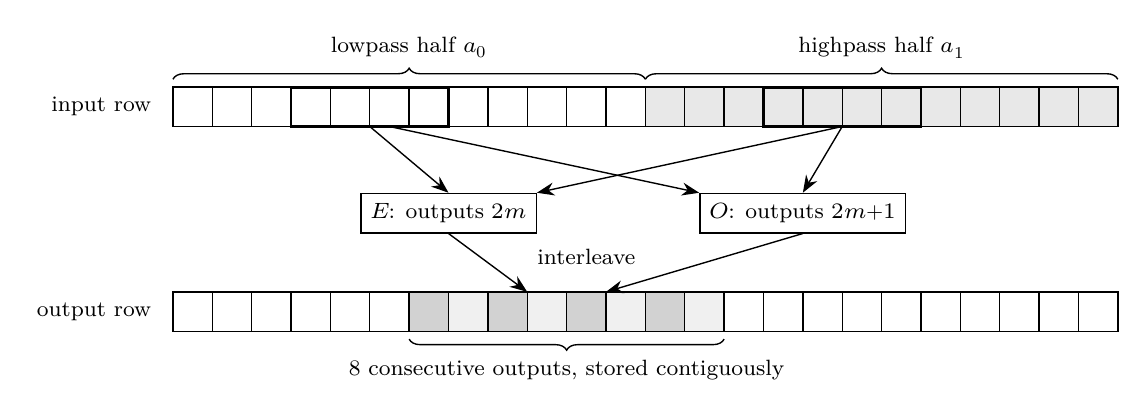
\begin{tikzpicture}[x=0.5cm,y=-0.5cm,font=\footnotesize]
  % input row: lowpass half then highpass half
  \foreach \i in {0,...,11} \draw (\i,0) rectangle (\i+1,1);
  \foreach \i in {12,...,23} \draw[fill=gray!18] (\i,0) rectangle (\i+1,1);
  \node[anchor=east] at (-0.3,0.5) {input row};
  \draw[decorate,decoration={brace,amplitude=4pt}] (0,-0.2) -- (12,-0.2) node[midway,above=4pt] {lowpass half $a_0$};
  \draw[decorate,decoration={brace,amplitude=4pt}] (12,-0.2) -- (24,-0.2) node[midway,above=4pt] {highpass half $a_1$};
  % a vector of 4 consecutive m in each half
  \draw[line width=1pt] (3,0) rectangle (7,1);
  \draw[line width=1pt] (15,0) rectangle (19,1);
  % even and odd vectors
  \node[draw,minimum width=2cm,minimum height=5mm] (E) at (7,3.2) {$E$: outputs $2m$};
  \node[draw,minimum width=2cm,minimum height=5mm] (O) at (16,3.2) {$O$: outputs $2m{+}1$};
  \draw[->] (5,1) -- (E.north);
  \draw[->] (17,1) -- (E.north east);
  \draw[->] (5.5,1) -- (O.north west);
  \draw[->] (17,1) -- (O.north);
  % interleaved output
  \foreach \i in {0,...,23} \draw (\i,5.2) rectangle (\i+1,6.2);
  \foreach \i in {6,8,...,12} \fill[gray!35] (\i,5.2) rectangle (\i+1,6.2);
  \foreach \i in {7,9,...,13} \fill[gray!12] (\i,5.2) rectangle (\i+1,6.2);
  \foreach \i in {6,...,13} \draw (\i,5.2) rectangle (\i+1,6.2);
  \node[anchor=east] at (-0.3,5.7) {output row};
  \draw[->] (E.south) -- (9,5.2);
  \draw[->] (O.south) -- (11,5.2);
  \node at (10.5,4.3) {interleave};
  \draw[decorate,decoration={brace,amplitude=4pt,mirror}] (6,6.4) -- (14,6.4) node[midway,below=4pt] {8 consecutive outputs, stored contiguously};
\end{tikzpicture}

  \caption{Row-direct synthesis: in the interior of a row, the even outputs $2m$ for four
  consecutive $m$ use the same terms shifted by one sample, and so do the odd ones; two vectors
  are computed and interleaved into eight consecutive outputs.}
  \label{fig:rowdirect}
\end{figure}

\subsection{Mixed float and double arithmetic}

NBIS mixes float and double in ways C's promotion rules make easy to miss. The codec mirrors
each case, and two of them could be vectorized in float only after a short proof.
\begin{itemize}
  \item \emph{Scaled integers}: NBIS converts the integer to float and divides by 10 once per
    exponent step, rounding to float after each division; the codec does the same.
  \item \emph{Dequantization}: NBIS adds $Z/2$ in double to a float product and rounds the sum to
    float. The double sum of two floats is exact when their exponents differ by fewer than 29,
    and then rounding it to float gives the correctly rounded float sum, which is what a float
    addition returns. Here the two terms differ by at most a factor of about $|p| \le 65535$, so
    a float addition gives NBIS's result.
  \item \emph{Quantization}: NBIS computes $(\text{short})(t + 1.0)$ in double for a quotient
    $t > 0$, and $(\text{short})(t - 1.0)$ for $t < 0$. Truncation commutes with adding one when the
    sign does not change, so $\mathrm{trunc}(t) \pm 1$ in float gives the same index, with one
    division per coefficient instead of two branches.
  \item \emph{Output}: NBIS adds $0.5$ in double before truncating; for the same reason as above,
    adding $0.5$ in float gives the same pixel.
\end{itemize}
The variance sums and the bit-allocation constant of the encoder keep NBIS's sequential float
accumulation and its double-precision \code{pow} and \code{log} calls, which on Linux resolve to
the same C library NBIS uses.

\subsection{Verification}

Table~\ref{tab:verification} lists what the test suite checks against NBIS. The expected outputs
are 64-bit hashes of what NBIS produced, stored in the repository, so the tests need the public
NIST data but not NBIS itself.

\begin{table}[ht]
  \centering\small
  \begin{tabular}{@{}p{7.4cm}p{6.4cm}@{}}
    \toprule
    check & result \\
    \midrule
    exact decoder, 86 NIST decoder files (9/7, 6/10, 10/10 and 9/11 filter banks), every
    backend (AVX-512 on the server of Section~\ref{sec:server}), 1 and 4 threads & identical pixels in every case \\
    exact encoder, 40 images at 0.75 and 2.25 bits per pixel, every backend & identical bytes in all 80 cases \\
    quantizer indices of the two NIST reference files & identical in all 60 subbands \\
    WebAssembly build (scalar and SIMD), three images & identical pixels \\
    fast decoder against NBIS, 86 files & Annex AA.3 met in every case (at least 99.994\% equal, never more than 1 apart) \\
    fast encoder against NBIS, 80 cases & Annex AA.2 met in every case (size within 0.04\%, bins within 0.015\%) \\
    \bottomrule
  \end{tabular}
  \caption{Exactness checks of the test suite (\code{cargo test} with \code{WSQ\_NIST\_DIR} set).}
  \label{tab:verification}
\end{table}

\section{The optimizations, one by one}
\label{sec:optimizations}

The first working version already decoded image \texttt{a002} seven times faster than NBIS,
because it vectorized the transform from the start. Table~\ref{tab:history} follows the decoder
from there; each row was measured right after the change, on the same image and core, so the
numbers carry the noise of separate runs (a few percent). Two changes that did not pay are
listed as well.

\begin{table}[ht]
  \centering\small
  \begin{tabular}{@{}rp{9.6cm}rr@{}}
    \toprule
    & change & AVX2 (ms) & vs NBIS \\
    \midrule
    0 & NBIS 5.0.0, for reference & 53.5 & 1.0$\times$ \\
    1 & first version: NBIS schedules evaluated across lines, transposes for the row pass & 7.59 & 7.0$\times$ \\
    2 & schedules cached per image size; buffers reused; pixel conversion vectorized & 6.17 & 8.7$\times$ \\
    3 & entropy decoding writes straight into the coefficient array & 5.78 & 9.3$\times$ \\
    -- & eight accumulators instead of four in the column kernel (no effect, reverted) & 5.86 & \\
    4 & row-direct synthesis, two dependency chains (no effect) & 6.07 & \\
    5 & row-direct synthesis, eight dependency chains & 5.16 & 10.4$\times$ \\
    -- & template column kernel (slower with 8 lanes; kept for 4-lane backends only) & 5.45 & \\
    6 & column kernel chosen by vector width & 4.55 & 11.8$\times$ \\
    7 & entropy decoding into a linear buffer without branches, vector dequantization & 4.48 & 11.9$\times$ \\
    8 & four threads: three entropy-coded blocks and the large splits in parallel & 2.47 & 21.7$\times$ \\
    \bottomrule
  \end{tabular}
  \caption{Decoding \texttt{a002} at 0.75 bits per pixel, exact mode, AVX2, as the decoder evolved.}
  \label{tab:history}
\end{table}

\subsection{Fixed costs}

The first profile (stage times of version 1) showed 0.64~ms spent building the transform
schedules, 1.19~ms converting coefficients to pixels with scalar code and a fresh 5.8~MB
coefficient array per image, whose page faults spread over the other stages. Caching the
schedules by line length and filter bank, keeping the buffers in the decoder object, and a
vector pixel kernel brought the first 1.4~ms down.

\subsection{Entropy decoding}

Huffman decoding is sequential within a block: each code's length is known only after it is
read. A bare loop that decodes symbols and discards them runs at 3.3~ns per symbol, but placing
the symbols cost another 4.4~ns: the symbol type (a run of zeros or a value) is unpredictable,
and every value write needed the bookkeeping of which subband row it belonged to. Two changes
fixed this.
\begin{enumerate}
  \item A 10-bit lookup table whose entries hold the code length, the symbol's kind and its
    value, so that 98\% of the symbols cost one table load (codes longer than 10 bits, about
    2\%, take a slower path).
  \item A first pass that writes indices, in stream order, into a linear buffer with one code
    path for runs and values (Algorithm~\ref{alg:entropy}), and a second, vectorized pass that
    dequantizes each subband row into its place in the coefficient array, without branches.
\end{enumerate}
The entropy stage of \texttt{a002} went from 1.62~ms to 0.63~ms (2.6$\times$); at 2.25 bits per
pixel, with four times the symbols, from 5.78~ms to 2.40~ms.

\begin{algorithm}[ht]
  \caption{Branch-free placement of decoded symbols.}
  \label{alg:entropy}
  \begin{algorithmic}[1]
    \Require a block's entropy-coded bits; a zeroed buffer $L$ with one spare slot; range $[k_0, k_1)$
    \State $k \gets k_0$
    \While{$k < k_1$}
      \State $(\ell, \mathit{kind}, v) \gets \mathrm{LUT}[\text{next 10 bits}]$;\ consume $\ell$ bits \Comment{rare: long codes, escapes}
      \State $\mathit{run} \gets v$ \textbf{if} $\mathit{kind} = \text{run}$ \textbf{else} $0$;\quad $\mathit{val} \gets v$ \textbf{if} $\mathit{kind} = \text{value}$ \textbf{else} $0$
      \State $k \gets k + \mathit{run}$
      \State $L[k] \gets \mathit{val}$ \Comment{a run writes a zero where the next value goes}
      \State $k \gets k + [\mathit{val} \ne 0]$
    \EndWhile
  \end{algorithmic}
\end{algorithm}

\subsection{The inverse transform}

After the fixed costs, the transform took two thirds of the time, and the vector version was
only twice as fast as the scalar one with eight lanes. Two experiments located the problem.
Replacing every schedule by the identity, which leaves only the data movement, cost 2.5 of the
4.0~ms: the transform is limited by moving data, not by arithmetic. And the fast mode, which
does half the multiplications, was not faster. With the identity schedules, the row pass,
which transposed blocks of eight rows into a scratch buffer and back, cost twice as much as the
column pass.

The row-direct kernel (Section~\ref{sec:exactness}) removed the transposes of the synthesis but
was not faster at first: each output accumulates about eight products, every addition waits
four cycles for the previous one, and only two chains (even and odd) were in flight. Evaluating
four vectors of each parity at once gives eight independent chains and brought the transform of
\texttt{a002} from 3.99 to 3.13~ms. The same trick made the column pass slower on AVX2, where
the strip of 64 columns already provides enough independent work, so each backend uses the
kernel that suits its width. Fusing the column and the row pass of a split, so that the
intermediate stays in cache, was considered and rejected: synthesis cannot run in place (the
lowpass and highpass halves are read far from where the outputs go), and the copy it would need
moves as much data as it saves.

\subsection{Threads}

Inside one image, the three entropy-coded blocks of encoder number two are independent, and
their positions in the linear buffer are known from the subband sizes, so three threads decode
them. The transform's large splits (the image and its quadrants) share columns and then rows
among threads, separated by a barrier; the small, deep splits run on one thread, where
synchronization would cost more than the work.

\subsection{The encoder}

The same ideas, plus four specific to encoding: quantization divides once per coefficient with
the truncation identity of Section~\ref{sec:exactness} instead of branching per sign (0.72 to
0.27~ms on \texttt{cmp00001}); normalization converts bytes to floats eight at a time; the
tokenizer skips zeros a vector at a time, testing eight or sixteen coefficients with one
comparison; and the bit writer emits code and extra bits in one call and four bytes at a time.
The encoder of \texttt{a002} went from 10.3~ms in its first version to 6.9~ms.

\section{Results}
\label{sec:results}

\subsection{Decoding and encoding on one core}

Tables~\ref{tab:decode} and~\ref{tab:encode} sum the per-image times over the 40 images. With
AVX2, decoding is about 11 times faster than NBIS and encoding 4 to 6 times; SSE2, which every
x86-64 processor has, keeps 9 and 4 times. Even the scalar backend is more than five times
faster than NBIS at decoding: most of the gain comes from the algorithms (cached schedules,
branch-free entropy decoding, fewer passes over memory), not from the vector width.

% Generated by tools/gen_tables.py; do not edit by hand.
\begin{table}[ht]
  \centering\small
  \begin{tabular}{@{}lrrrrrr@{}}
    \toprule
    & \multicolumn{3}{c}{0.75 bits per pixel} & \multicolumn{3}{c}{2.25 bits per pixel}\\
    \cmidrule(lr){2-4}\cmidrule(l){5-7}
    implementation & total (ms) & Mpx/s & speedup & total (ms) & Mpx/s & speedup\\
    \midrule
    NBIS 5.0.0 (C) & 1\,404 & 28 & 1.0$\times$ & 1\,622 & 24 & 1.0$\times$\\
    scalar, exact & 253 & 153 & 5.5$\times$ & 284 & 137 & 5.7$\times$\\
    scalar, fast & 226 & 172 & 6.2$\times$ & 258 & 150 & 6.3$\times$\\
    SSE2, exact & 155 & 250 & 9.0$\times$ & 179 & 216 & 9.0$\times$\\
    SSE2, fast & 154 & 252 & 9.1$\times$ & 179 & 217 & 9.1$\times$\\
    AVX2, exact & 119 & 325 & 11.8$\times$ & 150 & 259 & 10.8$\times$\\
    AVX2, fast & 120 & 324 & 11.7$\times$ & 149 & 260 & 10.9$\times$\\
    \bottomrule
  \end{tabular}
  \caption{Decoding the 40 NBIS-encoded images of the NIST set (41.0 megapixels in all), one core: sum of the per-image medians, throughput and speedup over NBIS.}
  \label{tab:decode}
\end{table}

% Generated by tools/gen_tables.py; do not edit by hand.
\begin{table}[ht]
  \centering\small
  \begin{tabular}{@{}lrrrrrr@{}}
    \toprule
    & \multicolumn{3}{c}{0.75 bits per pixel} & \multicolumn{3}{c}{2.25 bits per pixel}\\
    \cmidrule(lr){2-4}\cmidrule(l){5-7}
    implementation & total (ms) & Mpx/s & speedup & total (ms) & Mpx/s & speedup\\
    \midrule
    NBIS 5.0.0 (C) & 1\,080 & 36 & 1.0$\times$ & 1\,210 & 32 & 1.0$\times$\\
    scalar, exact & 442 & 88 & 2.4$\times$ & 495 & 78 & 2.4$\times$\\
    scalar, fast & 370 & 105 & 2.9$\times$ & 425 & 91 & 2.8$\times$\\
    SSE2, exact & 278 & 140 & 3.9$\times$ & 341 & 114 & 3.6$\times$\\
    SSE2, fast & 221 & 175 & 4.9$\times$ & 288 & 135 & 4.2$\times$\\
    AVX2, exact & 242 & 160 & 4.5$\times$ & 313 & 124 & 3.9$\times$\\
    AVX2, fast & 186 & 209 & 5.8$\times$ & 251 & 155 & 4.8$\times$\\
    \bottomrule
  \end{tabular}
  \caption{Encoding the 40 images of the NIST set at two target rates, one core.}
  \label{tab:encode}
\end{table}


Table~\ref{tab:stages} breaks the times of \texttt{a002} into stages. The inverse transform
still dominates decoding (about 3.2 of 4.8~ms); entropy decoding and dequantization take
1.0~ms together. In the encoder, the forward transform takes half the time and the tokenizer is
the next largest stage.

% Generated by tools/gen_tables.py; do not edit by hand.
\begin{table}[ht]
  \centering\small
  \begin{tabular}{@{}lrrrrrrr@{}}
    \toprule
    decoder & parse & zero & entropy & dequantize & plan & transform & output\\
    \midrule
    scalar, exact & 0.03 & 0.21 & 0.62 & 0.37 & 0.01 & 7.37 & 1.13\\
    AVX2, exact & 0.03 & 0.22 & 0.63 & 0.37 & 0.01 & 3.17 & 0.34\\
    AVX2, fast & 0.03 & 0.21 & 0.62 & 0.34 & 0.01 & 2.96 & 0.31\\
    \midrule
    encoder & normalize & transform & variance & quantize & tokenize & tables & entropy\\
    \midrule
    scalar, exact & 0.47 & 8.84 & 0.19 & 2.72 & 1.57 & 0.19 & 0.39\\
    AVX2, exact & 0.43 & 3.84 & 0.18 & 0.61 & 1.27 & 0.19 & 0.39\\
    AVX2, fast & 0.42 & 3.98 & 0.19 & 0.61 & 1.30 & 0.19 & 0.39\\
    \bottomrule
  \end{tabular}
  \caption{Median time of each stage, in milliseconds, for image \texttt{a002} at 0.75 bits per pixel. Decoder: \emph{zero} clears the index buffer, \emph{plan} fetches the cached transform schedules. Encoder: \emph{entropy} writes the bit stream; table building and tokenizing are separate.}
  \label{tab:stages}
\end{table}


\subsection{Threads and batches}

A single image decodes 1.7 times faster with four threads (Table~\ref{tab:threads}); the
serial parts (the deep splits, the largest entropy-coded block) limit the gain, and small
images gain little. Batches scale better, since images are independent: on the four performance
cores, 829 images per second, against 319 on one core (Table~\ref{tab:batch}). Eight threads
(the performance cores with both their hardware threads) reach 934; twelve, adding the
efficiency cores, are slower, because the transform saturates memory bandwidth.

% Generated by tools/gen_tables.py; do not edit by hand.
\begin{table}[ht]
  \centering\small
  \begin{tabular}{@{}lrrrr@{}}
    \toprule
    image & 1 thread & 2 threads & 4 threads & 8 threads\\
    \midrule
    \texttt{cmp00001} (589$\times$605) & 0.96 & 0.95 & 0.79 & 0.84\\
    \texttt{a002} (1452$\times$1006) & 4.63 & 3.94 & 2.66 & 2.73\\
    \texttt{sample\_19} (1600$\times$1500) & 7.69 & 6.63 & 4.58 & 4.42\\
    \bottomrule
  \end{tabular}
  \caption{Decoding one image with several threads (AVX2, exact): median milliseconds. Threads beyond four share the four performance cores.}
  \label{tab:threads}
\end{table}

% Generated by tools/gen_tables.py; do not edit by hand.
\begin{table}[ht]
  \centering\small
  \begin{tabular}{@{}lrrrrr@{}}
    \toprule
    threads & 1 & 2 & 4 & 8 & 12\\
    \midrule
    exact, images/s & 319 & 530 & 829 & 934 & 843\\
    exact, Mpx/s & 309 & 513 & 803 & 904 & 817\\
    fast, images/s & 312 & 520 & 790 & 856 & 839\\
    fast, Mpx/s & 302 & 504 & 765 & 829 & 813\\
    \bottomrule
  \end{tabular}
  \caption{Batch decoding of the 40 images at 0.75 bits per pixel, one image per thread (AVX2). Without the inverse transform (entropy decoding and dequantization only), four threads reach 3\,093 images/s.}
  \label{tab:batch}
\end{table}


\subsection{WebAssembly}

The extension runs the codec as WebAssembly. With SIMD the WebAssembly build is 1.35 times
slower than native AVX2 and still eight times faster than native NBIS; without SIMD it is about
three times slower than with it (Table~\ref{tab:wasm}). Its outputs are identical to NBIS's: WebAssembly
float arithmetic follows IEEE 754 exactly, and the exact kernels use no fused operations.

% Generated by tools/gen_tables.py; do not edit by hand.
\begin{table}[ht]
  \centering\small
  \begin{tabular}{@{}lrrrr@{}}
    \toprule
    image & NBIS (C) & native AVX2 & wasm scalar & wasm SIMD\\
    \midrule
    \texttt{cmp00001} & 12.31 & 0.96 & 4.62 & 1.54\\
    \texttt{a002} & 52.38 & 4.80 & 18.67 & 6.50\\
    \texttt{sample\_19} & 86.51 & 7.65 & 29.14 & 10.74\\
    \bottomrule
  \end{tabular}
  \caption{Decoding in WebAssembly (Node.js 24, one core), exact mode, median milliseconds; the WebAssembly outputs are identical to those of NBIS.}
  \label{tab:wasm}
\end{table}


\subsection{A server processor with AVX-512}
\label{sec:server}

The laptop has no AVX-512, so the test suite and the single-core measurements were repeated on a
server processor that has it, an Intel Xeon Gold 6330, which other users shared at the time.
Every test passes there with AVX-512 among the backends: the exact decoder reproduces NBIS on the
86 decoder files with 1 and 4 threads, and the exact encoder writes NBIS's bytes in the 80 cases.

Table~\ref{tab:server} gives the times. Doubling the vector width from AVX2 to AVX-512 gains
little, as expected from a transform limited by data movement (Section~\ref{sec:optimizations}).
In four rounds that alternated the two backends on the same core, exact decoding was 8 to 15\%
faster with AVX-512 in every round and exact encoding 2 to 8\% (one round, at 27\%, was an
outlier); fast decoding and fast encoding showed no consistent difference. The absolute times
varied by up to 20\% between rounds, because of the other jobs on the server, so only the ratios
within a round are reliable. A server core is slower than the laptop's performance core (NBIS takes
2.5~s for the set against 1.4~s), but the speedup over NBIS is similar: about 12 to 13 times at
decoding and 4.5 to 5.7 times at encoding.

% Generated by tools/gen_tables.py; do not edit by hand.
\begin{table}[ht]
  \centering\small
  \begin{tabular}{@{}lrrrrrr@{}}
    \toprule
    & \multicolumn{3}{c}{decode} & \multicolumn{3}{c}{encode}\\
    \cmidrule(lr){2-4}\cmidrule(l){5-7}
    implementation & total (ms) & vs NBIS & vs AVX2 & total (ms) & vs NBIS & vs AVX2\\
    \midrule
    NBIS 5.0.0 (C) & 2\,546 & 1.0$\times$ & 0.08 & 1\,775 & 1.0$\times$ & 0.22\\
    scalar, exact & 477 & 5.3$\times$ & 0.43 & 754 & 2.4$\times$ & 0.53\\
    scalar, fast & 439 & 5.8$\times$ & 0.47 & 652 & 2.7$\times$ & 0.61\\
    SSE2, exact & 253 & 10.1$\times$ & 0.81 & 470 & 3.8$\times$ & 0.85\\
    SSE2, fast & 260 & 9.8$\times$ & 0.79 & 419 & 4.2$\times$ & 0.95\\
    AVX2, exact & 205 & 12.4$\times$ & 1.00 & 397 & 4.5$\times$ & 1.00\\
    AVX2, fast & 193 & 13.2$\times$ & 1.06 & 312 & 5.7$\times$ & 1.28\\
    AVX-512, exact & 188 & 13.5$\times$ & 1.09 & 391 & 4.5$\times$ & 1.02\\
    AVX-512, fast & 196 & 13.0$\times$ & 1.05 & 312 & 5.7$\times$ & 1.28\\
    \bottomrule
  \end{tabular}
  \caption{The same measurements on a server processor with AVX-512 (Intel Xeon Gold 6330, one core): the 40 images of the NIST set at 0.75 bits per pixel, sum of the per-image medians. \emph{vs AVX2} is the speed relative to the exact AVX2 backend on the same core.}
  \label{tab:server}
\end{table}


\section{Does giving up exactness pay?}
\label{sec:relaxation}

% Generated by tools/gen_tables.py; do not edit by hand.
\newcommand{\varexact}{4.13}\newcommand{\varfast}{0.36}\newcommand{\encexact}{14.5}\newcommand{\encfast}{10.9}


The fast mode is free to reorder operations, fold symmetric filter taps (halving the
multiplications), use fused multiply-add and compute in double precision where that is cheaper.
Table~\ref{tab:relax} compares it with the exact mode stage by stage.

% Generated by tools/gen_tables.py; do not edit by hand.
\begin{table}[ht]
  \centering\small
  \begin{tabular}{@{}llrrr@{}}
    \toprule
    & stage & exact (ms) & fast (ms) & fast / exact\\
    \midrule
    decoder & entropy & 15 & 15 & 1.00\\
     & dequantize & 10 & 10 & 1.00\\
     & transform & 80 & 81 & 1.01\\
     & output & 8 & 8 & 0.94\\
     & total & 119 & 120 & 1.00\\
    \midrule
    encoder & normalize & 12 & 11 & 0.98\\
     & transform & 106 & 102 & 0.96\\
     & variance & 63 & 9 & 0.14\\
     & quantize & 17 & 17 & 1.00\\
     & total & 242 & 186 & 0.77\\
    \bottomrule
  \end{tabular}
  \caption{Exact against fast arithmetic, AVX2, summed over the 40 images at 0.75 bits per pixel (one core).}
  \label{tab:relax}
\end{table}


\paragraph*{Decoding: no.} With AVX2 the two modes take the same time to the percent. The
transform is limited by data movement (Section~\ref{sec:optimizations}), so doing half the
multiplications changes nothing; dequantization and pixel conversion are memory-bound as well.
Only the scalar backend, which is compute-bound, gains (11\% over the 40 images,
Table~\ref{tab:decode}). Since exactness costs nothing in the configurations that matter
(AVX2 natively, SIMD in WebAssembly), the decoder defaults to exact mode.

\paragraph*{Encoding: yes, in one place.} The encoder is 23\% faster in fast mode over the set,
and almost all of the difference is the subband variances. NBIS sums them in float, one
coefficient after the other; reproducing its rounding forces the same sequential sum, a chain
of dependent additions that no vector unit can shorten. The fast mode sums in double with
independent accumulators. On images whose variance is estimated over whole subbands (7 of the
40, after the version 3.1 rule), the difference is large: \texttt{sample\_19} spends
\varexact~ms on variances in exact mode and \varfast~ms in fast mode, and encodes in \encfast~ms
instead of \encexact~ms. The fast encoder's files meet every encoder criterion of Annex AA
against NBIS.

\paragraph*{What else could a relaxed mode do?} Lifting would cut the arithmetic of the 9/7
transform further, but arithmetic is not the bottleneck. Storing the intermediate of each split
in 16-bit floats would halve the data movement that is, at the cost of precision; that and
integer arithmetic remain untested.

\section{A GPU for batch decoding}
\label{sec:gpu}

Entropy decoding is sequential within a block, but the inverse transform is massively
parallel, so a GPU could take it over while the CPU decodes the entropy-coded data of the next
images. The test split the work that way:
\begin{itemize}
  \item the CPU parses, entropy-decodes and dequantizes (\code{Decoder::decode\_coefficients});
  \item the GPU receives the coefficient array, runs the inverse transform (the specification's
    formulas, one indexed gather and multiply-add per filter tap, fused into one kernel per pass
    by \code{torch.compile}) and converts to pixels, for batches of images of the same size;
  \item copies to and from the GPU overlap with computation (two CUDA streams, double buffers).
\end{itemize}
The GPU is the laptop's GeForce RTX 3050 (6~GB, 20 multiprocessors, PCIe~4 at about
8.7~GB/s measured). Its results match the exact decoder within the Annex AA.3 tolerance
(99.998\% of the pixels equal, none off by more than one) but not bit for bit.

\begin{table}[ht]
  \centering\small
  \begin{tabular}{@{}lrr@{}}
    \toprule
    images per second & \texttt{a002} (1452$\times$1006) & \texttt{cmp00001} (589$\times$605) \\
    \midrule
    CPU, full decode, 1 thread & 214 & 950 \\
    CPU, full decode, 8 threads & 604 & 3\,689 \\
    CPU, coefficients only, 4 threads & 1\,859 & 11\,181 \\
    GPU, transform and pixels only (batch 16 / 32) & 850 & 3\,409 \\
    GPU, upload of float32 coefficients alone & 1\,493 & 6\,100 \\
    GPU, transform with copies, overlapped & 723 & 2\,993 \\
    \bottomrule
  \end{tabular}
  \caption{Batch decoding on the CPU and with the transform on the laptop GPU.}
  \label{tab:gpu}
\end{table}

Table~\ref{tab:gpu} gives the answer for this machine: the GPU roughly matches the optimized CPU
path. For large images it is 20\% faster (723 against 604 images per second); for smaller ones
the CPU wins (3\,689 against 2\,993). The main value of the GPU here would be to leave the CPU
free. Three limits stand out.
\begin{itemize}
  \item \emph{Memory bandwidth}: the gathers of the compiled passes reach 110~GB/s, close to what
    the laptop GPU sustains on a plain copy (155~GB/s).
  \item \emph{The bus}: float32 coefficients take 4 bytes per pixel, and uploading them alone
    caps the rate at about 1\,500 images per second; sending the 16-bit quantizer indices and
    dequantizing on the GPU would halve that.
  \item \emph{The CPU part}: entropy decoding and dequantization reach about 1\,860 images of this
    size per second on four cores, so a faster GPU would soon wait for the CPU.
\end{itemize}
A data-center GPU has 15 to 20 times the memory bandwidth of this one and a faster bus; on a
server with many cores for the entropy decoding, offloading the transform should then pay
clearly. That test (for instance on the H100 of the research group) is left for later.

\section{Limitations and next steps}
\label{sec:limitations}

\begin{itemize}
  \item \emph{ARM NEON} is not implemented; on ARM the scalar backend runs. AVX-512 was tested
    on a single server processor.
  \item \emph{The inverse transform} remains limited by data movement. Processing two tree levels
    per pass, or (in fast mode) keeping intermediates in 16-bit floats, could reduce it.
  \item \emph{Entropy decoding} is sequential within a block; streams with more than three blocks
    are decoded on one thread.
  \item \emph{Times} come from a laptop processor, whose frequency varies with temperature, and
    from a shared server; medians of several runs reduce, but do not remove, that noise.
\end{itemize}

\begin{thebibliography}{9}
\small

\bibitem{algorithm}
J.~F.~Contreras.
\emph{The WSQ Fingerprint Image Compression Algorithm: a didactic description of the FBI
specification IAFIS-IC-0110 (version 3.1)}. \texttt{docs/algorithm} in the \texttt{wsq-viewer}
repository, 2026.

\bibitem{wsq31}
Federal Bureau of Investigation, Criminal Justice Information Services Division.
\emph{WSQ Gray-scale Fingerprint Image Compression Specification}, IAFIS-IC-0110 (V3.1), 2010.

\bibitem{nbis}
National Institute of Standards and Technology.
\emph{NIST Biometric Image Software (NBIS)}, release 5.0.0, 2015.

\bibitem{nistcert}
National Institute of Standards and Technology.
\emph{WSQ Certification Procedure} and reference image data set version 2.0.
\url{https://www.nist.gov/programs-projects/wsq-certification-procedure}

\end{thebibliography}


\end{document}
